\textbf{{1. 按下标访问顺序表元素}}

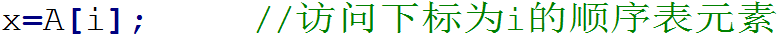
\includegraphics[width=2.18750in,height=0.10417in]{png-jpeg-pics/98374E4A1099338D04981D1ACB6B6417.png}

\textbf{{2. 按元素值的查找算法}}

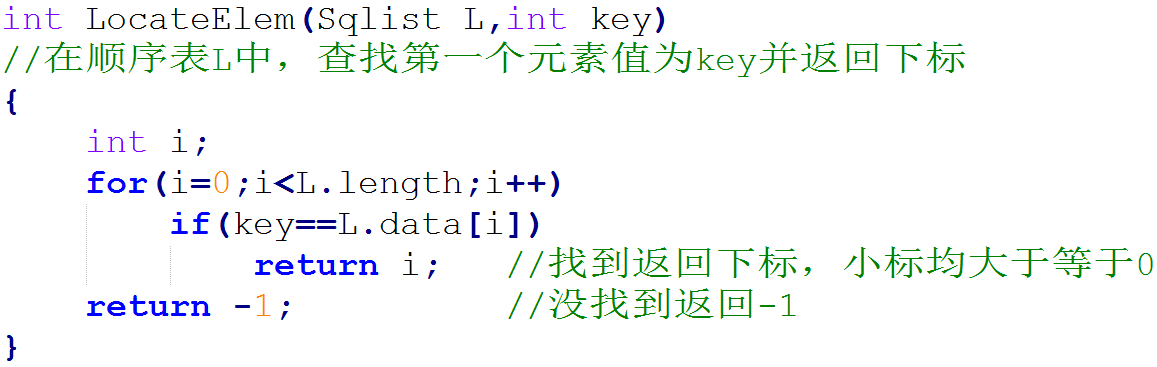
\includegraphics[width=3.33333in,height=1.06250in]{png-jpeg-pics/2F1E51D3E4237550D9FDD9DA8D0C128A.png}

\textbf{{3. 插入数据元素的算法}}

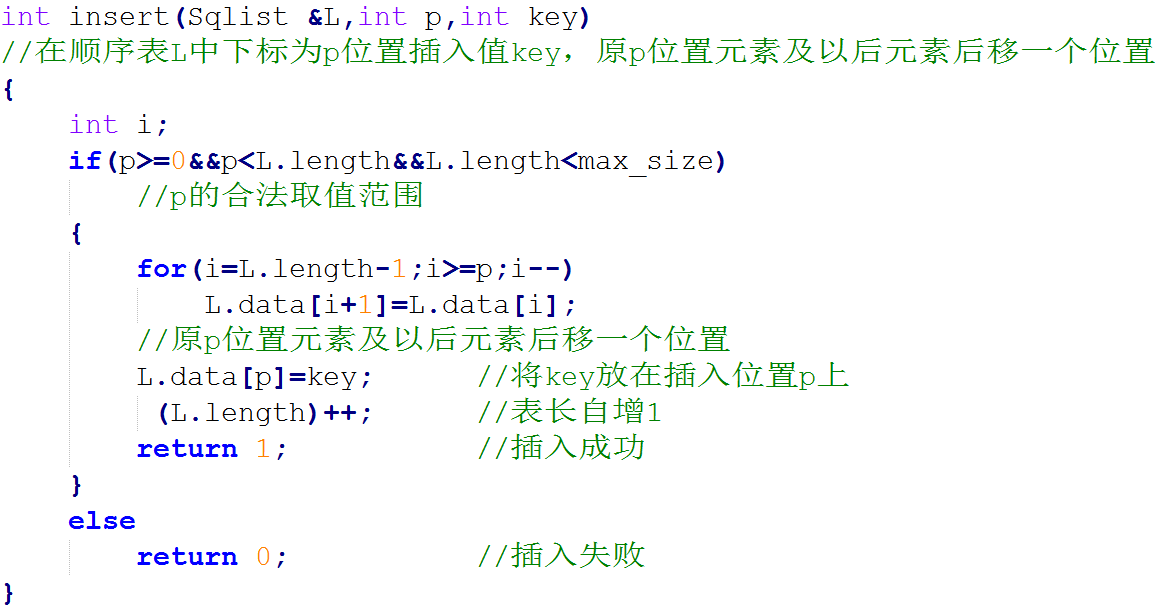
\includegraphics[width=3.33333in,height=1.75000in]{png-jpeg-pics/CD4FB43A8A96D42B741B32A293CA4082.png}

\textbf{{4. 删除数据元素的算法}}

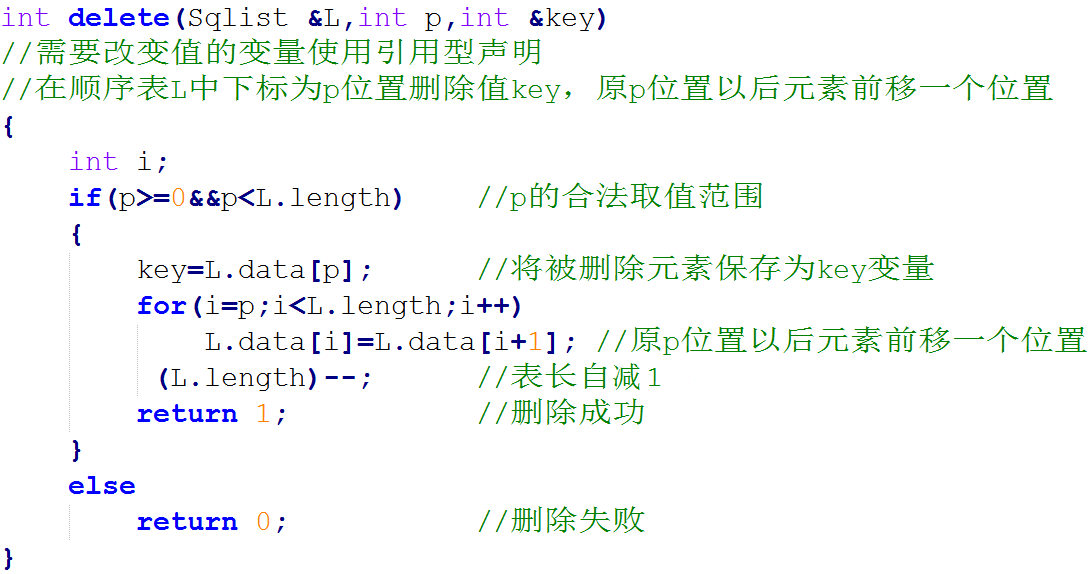
\includegraphics[width=3.12500in,height=1.64583in]{png-jpeg-pics/7633470FDBFBF6732CD62D088DFDF1A2.png}
